\subsection{Uso de Arduino y ESP32}

Arduino es una placa de desarrollo de hardware libre, que puede ser utilizada tanto por aficionados como por fabricantes para diseñar y construir dispositivos que interactúen con el mundo real, a través de una gran cantidad de sensores y otros elementos electrónicos que están disponibles en el mercado. Aunque utilizamos el término Arduino para referirnos a un tipo específico de placa de desarrollo, también se usa para hablar de la empresa que fabrica estas placas o para describir a la comunidad en torno a las diferentes placas compatibles \cite{pena}.

\textbf{Clasificación Dse Pines}

\subsubsection{Pines analógicos}
Los pines analógicos pueden leer un amplio rango de valores, por lo que son útiles para realizar un control más detallado de las lecturas obtenidas. En general se encuentran 6 pines y mediante estos pines es posible obtener datos de sensores en forma de variaciones continuas de un voltaje. 

\subsubsection{Pines digitales}
Los pines digitales son capaces de leer y escribir un solo estado, es decir, encendido o apagado. En la mayoría de las placas Arduino hay 14 pines \cite{pena}.

\begin{figure}[H]
     \centering
     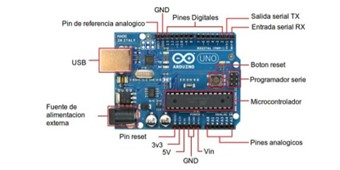
\includegraphics[scale = 0.97]{Imagenes/ardr3.jpg}
     \caption{Arduino UNO R3}{Fuente: Adaptado de ~\cite{mecafenix}}
\end{figure}

\textbf{ESP32}

Plataforma de  hardware  abierto, basada   en   un   sistema  en  chip  (SoC,  del  inglés  System on  a  Chip) con hardware específico para comunicaciones inalámbricas, entre otros recursos. Este  permite  el  desarrollo  de  aplicaciones  en  diferentes  lenguajes  de  programación,  frameworks, bibliotecas  y  recursos  diversos.

El  SoC  ESP32  de  Espressif  Systems  es  la  evolución  del  ESP8266,  diseñado  para  superar  a  su  antecesor  en  capacidad  de  procesamiento  y  conectividad;  integra  un  potente  microcontrolador  con  arquitectu-ra de 32 bits, conectividad wifi y Bluetooth. El  sistema  en  el  módulo  (SoM,  del  inglés  System  on  Module)  ESP-32S  fabricado  por  Ai-Thinker  integra  en  un  módulo  el  SoC  ESP32, memoria FLASH, cristal oscilador y antena wifi en PCB.

\begin{figure}[htb]
    \centering
    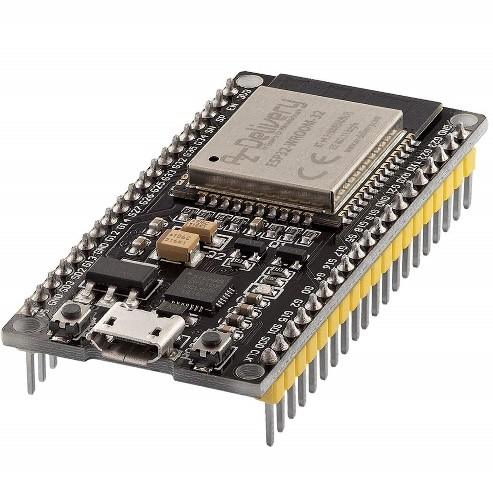
\includegraphics[scale = 0.50]{Imagenes/esp32cam.jpg}
    \caption{ESP32}{Fuente: Adaptado de ~\cite{delivery}}
\end{figure}

Se destaca el módulo ESP32-CAM, que incluye una cámara OV2640 y varios GPIO para conectar periféricos usando un ESP32. El módulo también cuenta con una ranura para tarjeta microSD, que permite almacenar imágenes tomadas de la cámara o almacenar archivos y viene con el módulo de cámara de 2MP. Las funcionalidades de este módulo y su capacidad de realizar diversas tareas lo han convertido en un componente eficaz para la seguridad. Este módulo se puede utilizar en videovigilancia para transmitir imágenes o funcionar como sensores en un sistema de visión \cite{salvador}.

\begin{figure}[htb]
    \centering
    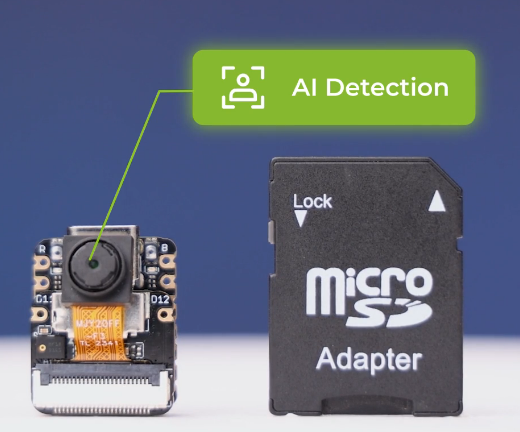
\includegraphics[scale = 0.50]{Imagenes/xiao esp32cam.png}
    \caption{XIAO ESP32 CAM}{Fuente: Adaptado de~\cite{foto_xiao}}
\end{figure}
